\documentclass{article}
% \VignettePackage{funtooNorm}
% \VignetteIndexEntry{Normalization of Illumina Infinium HumanMethylation450 Beadchip data}
\usepackage{graphicx}
\usepackage[margin=2cm]{geometry}
\usepackage[colorlinks=true,urlcolor=blue]{hyperref}
\usepackage{array}
\usepackage{color}
\usepackage{underscore}
%\usepackage[authoryear,round]{natbib}
\bibliographystyle{plainnat}
\usepackage{verbatim}
%\usepackage[utf8]{inputenc} % for UTF-8/single quotes from sQuote()
\usepackage{Sweave}%
% for bold symbols in mathmode
\usepackage{bm}
\usepackage{setspace}
\doublespacing



\title{Using funtooNorm}
\author{Celia Greenwood, Stepan Grinek, Kathleen Oros Klein}

\date{\today}
\sloppy
\hyphenpenalty 10000


\begin{document}
\input{funtooNorm-concordance}

\maketitle


%% Note: These are explained in '?RweaveLatex' :
%<<preliminaries, echo=FALSE>>=
%options(width=75)
%@

\section{Introduction}


The \textbf{funtooNorm} package provides  a function for normalization of Illumina Infinium Human Methylation 450 BeadChip (Illumina 450K) data when there are samples from multiple tissues or cell types. 
The algorithm in this package represents an extension of a normalization method introduced recently by
\cite{Fortin2014, Aryee2014}. 
In addition to the percentile-specific adjustments implemented in funNorm, funtooNorm is specifically designed to allow flexibility in the adjustments for different cell types or tissue types.  
Percentiles of methylation levels may vary across cell types and hence the original funNorm may not be ideal if applied to all samples simultaneously.  
Normalization separately for each cell type may introduce unwanted variability if sample sizes are small.
Therefore, this algorithm provides flexibility while optimizing the sample size used to estimate the corrections.

A partial least squares (PLS) fit is included as the core of the algorithm, followed by smoothing across percentiles. 

Note that the current version of the package does not do a good job of normalizing the Y chromosome probes; the funNorm method performs better.  
In a subsequent version of the package we will address this issue. 

\section{Package use}

The user needs to provide the following information:
\begin{itemize}
  \item \verbatim{sigA, sigB:} Two matrices containing the signal A and signal B information from the IDAT files.
  These matrices should have columns representing each sample, and rows for each probe.  
  The probe names should index the rows, and the sample names should index the columns.
  These can be obtained from the Illumina IDAT files using Genome Studio  (http://www.illumina.com/applications/microarrays/microarray-software/genomestudio.html) by extracting Signal_A and Signal_B from the Sample Methylation Profile, or these can be obtained directly from the IDAT files with Bioconductor packages such as \textbf{illuminaio} and \textbf{IlluminaDataTestFiles}, \cite{Smith2013}. \textbf{illuminaio} provides the function readIDAT to extract signals from the IDAT files. Control probe signals can be extracted using probe summaries provided in file 4343238080_A_ProbeSummary.txt.gz of \textbf{IlluminaDataTestFiles}.
   \item \textbf{controlred, controlgrn:}  Two matrices containing the control probe signals, separately for the red and green channels. 
  The column labels (sample names) for each matrix should match the column labels of the signal A and signal B matrices.
  This information can also be extracted from the IDAT files using Genome Studio, by extracting Signal_Grn and Signal_Red from the Control Probe Profile or extracted directly from the IDAT files as described above.
   \item \textbf{cell\_type:} A list of the cell types or tissues, in the order corresponding to the columns of the signal A and signal B matrices.  
  There must be at least two different cell or tissue types in the data or the program will terminate with a warning.
\end{itemize}

The program also requires the following information, but default matrices are provided and used if the parameters are set to NULL in the function call.

\begin{itemize}
\item \textbf{Annot:} An annotation table, containing information on probe names, probe type, and color (for probes of type I).  
This can be extracted from the Illumina annotation information for the Infinium BeadChip.
A default annotation table is provided if not supplied including all probes on the 450K array.
\item  \textbf{cp.types:}  A list of the types of control probes to be used in the normalization.
\end{itemize}

Finally, a number of parameters control whether intermediate calculations should be stored, simply so that the analysis can be performed in stages if desired.

We have provided a small data set containing $N=93$ individuals and 20,000 probes to demonstrate the usage of the package. 
The samples are either from cord blood or foetal placenta tissue. 

Here is a basic call to normalize this sample data set: 
 %The code to be inserted
%\begin{Verbatim}
\begin{Schunk}
\begin{Sinput}
>     library(funtooNorm)
>     ncmp <- 4
>     funtoonormout <- funtoonorm(sigA=sigAsample, sigB=sigBsample, Annot=NULL, 
+                       controlred=matred, controlgrn=matgrn, 
+                       cp.types=NULL, cell_type = cell_type,
+                       ncmp=4, save.quant=TRUE, save.loess=TRUE, apply.loess=TRUE, validate=FALSE)
\end{Sinput}
\begin{Soutput}
Since Annot is NULL using default annotation. 
Since cp.types is NULL using default cp.types. 
Checking sanity of the data... 
Data is ok. 
\end{Soutput}
\begin{Sinput}
> 
\end{Sinput}
\end{Schunk}
%\end{Verbatim}

\emph{save.quant} implies that the quantiles should be saved;  \emph{save.loess} means that loess fits to the curves should be saved; \emph{apply.loess} means that the normalization itself should be applied to all the data based on the loess fits;  \emph{logit.quant} asks whether the quantiles should be logit-transformed prior to fitting PLS models.

An important user-chosen parameter is  \emph{ncmp}, the number of PLS components to be included in the model.  
This can be chosen after examining a series of fits with different numbers of PLS components, together with a cross-validation procedure to assess how well the quantiles are modelled by the control probe data.  
By setting $validate=N$, for a maximum of $N$ components, the algorithm will graph the cross-validated errors across the percentiles for
models with $1, 2, ... , N$ PLS components.  
Examination of these graphs will enable choice of the best value for \emph{ncmp} for each data set.

The following call performs cross-validation to assess the performance of the model fitting for \emph{ncmp} between 1 and 5.  
Note that here the \emph{ncmp} parameter is not specified.
%\begin{Verbatim}
\begin{Schunk}
\begin{Sinput}
>     #This call  will perform cross validation of to find optimal value of parameter ncmp for PLS regression:
>     funtoonormmout <- funtoonorm(sigA=sigAsample, sigB=sigBsample,
+                       controlred=matred, controlgrn=matgrn, 
+                       cp.types=cp.types, cell_type = cell_type,
+                       save.quant=TRUE, save.loess=TRUE, apply.loess=FALSE, validate=5)
\end{Sinput}
\begin{Soutput}
Since Annot is NULL using default annotation. 
Checking sanity of the data... 
Data is ok. 

 Starting validation with  5  PLS components... 
Done. Check your working directory for the file "validationCurves.pdf" 
\end{Soutput}
\begin{Sinput}
> 
\end{Sinput}
\end{Schunk}
%\end{Verbatim}

Calling the funtoonorm function with \emph{validate =N} produce set of plots, one for each type of probe and colour (probe type I red, signal A, ... probe type II, signal B).  By looking at figure \ref{val}, the goal is to choose the smallest value of \emph{ncmp} where the cross-validated error is small.
We have set 4 as the default value for \emph{ncmp}.
%%Add graph and explanations of its meaning.



\begin{figure}[val]
\centering
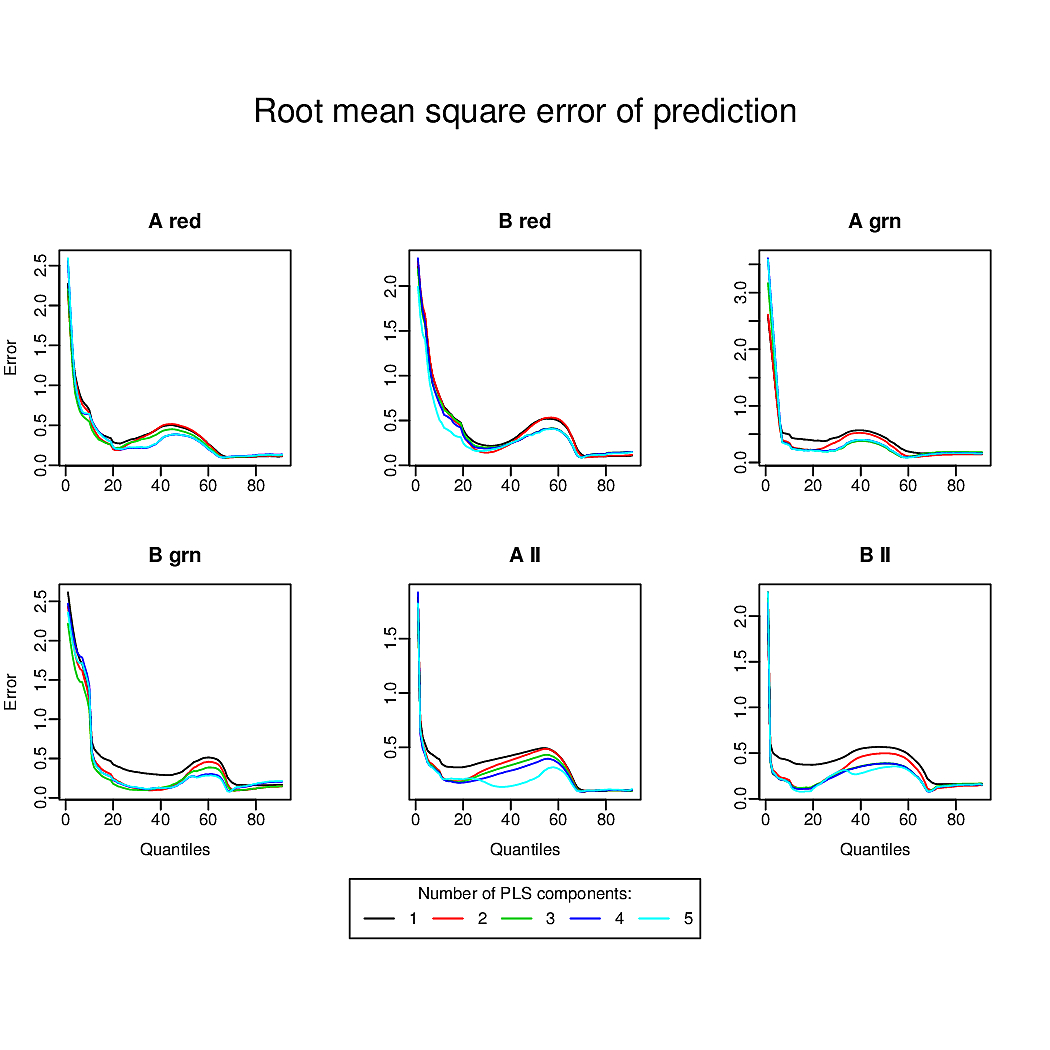
\includegraphics[width=10cm,height=10cm]{valid.jpg}
\caption{Cross-validated errors across percentiles of the signal distributions for different numbers of PLS components.  Top: signal A; Bottom: signal B;  Left: probe type I red; Middle: probe type I green; Right: probe type II.} \label{val}
\end{figure}


To access the performance of normalization function one can use a measure of intra-replicate differences \emph{M}, described in \cite{funntoNorm}. We provide a function \emph{agreement} implementing this measure. It takes as arguments a matrix of beta values and a vector of individual ID's. For the function to work some elements of individual's vector, obviously, should be identical. The returned value of \emph{M} is expected to be similar for the data before and after normalization:
%\begin{Verbatim}
\begin{Schunk}
\begin{Sinput}
> agreement(funtoonormout[[1]], individualID) # M for data before the normalization